%%% BEGIN UNIT
\wbunit{Partes iguales y fracciones}{Vas a aprender qué es una fracción cuando divides algo en partes iguales y cómo se lee y se escribe.}

\section{Repartos justos y partes iguales}

Ana y Beto van a compartir una pizza. Ana corta la pizza en $2$ partes iguales y le da una parte a Beto. Los dos reciben lo mismo. ¡Ese es un reparto justo!

\begin{center}
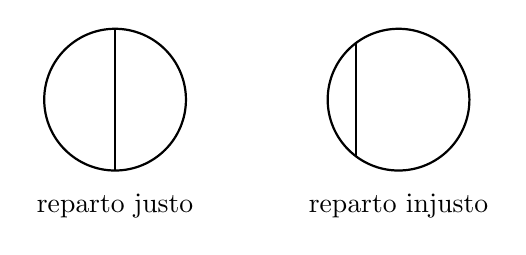
\begin{tikzpicture}[scale=0.9]
\draw[thick] (0,0) circle (1);
\draw[thick] (0,-1)--(0,1);
\node at (0,-1.5) {reparto justo};
\draw[thick] (4,0) circle (1);
\draw[thick] (3.4,-0.8)--(3.4,0.8);
\node at (4,-1.5) {reparto injusto};
\end{tikzpicture}
\end{center}

Ahora Ana corta la pizza en $2$ partes, pero una es grande y la otra es chica. Si cada uno recibe una parte, no reciben la misma cantidad. El reparto no es justo.

\begin{wbidea}[Partes iguales]
Cuando dividimos un entero (una pizza, un chocolate, una hoja de papel) en \textbf{partes iguales}, todas las partes tienen el mismo tamaño.

Para nombrar cada parte como un medio, un tercio o un cuarto, las partes deben ser iguales.
\end{wbidea}

\begin{wbexample}[¿Cuáles están en partes iguales?]
Observa las figuras. ¿Cuáles están divididas en partes iguales?

\begin{center}
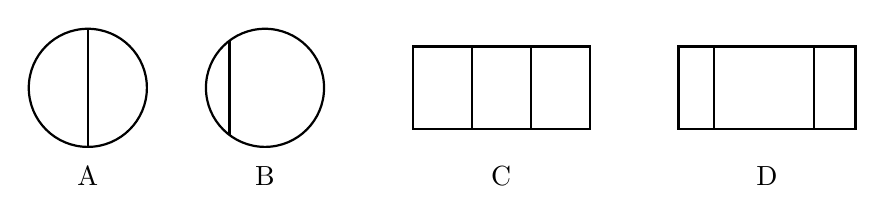
\begin{tikzpicture}[scale=0.75]
\draw[thick] (0,0) circle (1);
\draw[thick] (0,-1)--(0,1);
\node at (0,-1.5) {A};
\draw[thick] (3,0) circle (1);
\draw[thick] (2.4,-0.8)--(2.4,0.8);
\node at (3,-1.5) {B};
\draw[thick] (5.5,-0.7) rectangle (8.5,0.7);
\draw[thick] (6.5,-0.7)--(6.5,0.7);
\draw[thick] (7.5,-0.7)--(7.5,0.7);
\node at (7,-1.5) {C};
\draw[thick] (10,-0.7) rectangle (13,0.7);
\draw[thick] (10.6,-0.7)--(10.6,0.7);
\draw[thick] (12.3,-0.7)--(12.3,0.7);
\node at (11.5,-1.5) {D};
\end{tikzpicture}
\end{center}

\textbf{Paso 1.} Reviso la figura A. El círculo está cortado en $2$ partes y las dos tienen el mismo tamaño. Sí son iguales.

\textbf{Paso 2.} Reviso la figura B. El círculo está cortado en $2$ partes, pero la de la izquierda es más chica. No son iguales.

\textbf{Paso 3.} Reviso la figura C. El rectángulo está cortado en $3$ partes. Las tres tienen el mismo ancho y la misma altura. Sí son iguales.

\textbf{Paso 4.} Reviso la figura D. El rectángulo está cortado en $3$ partes, pero la primera es más angosta. No son iguales.

\textbf{Respuesta:} las figuras A y C están divididas en partes iguales.
\end{wbexample}

\begin{wbexample}[Un reparto justo]
Cuatro niños quieren compartir una barra de chocolate. ¿Cómo la divides para que el reparto sea justo?

\textbf{Paso 1.} Hay $4$ niños, así que necesito $4$ partes.

\textbf{Paso 2.} Las $4$ partes deben ser iguales, para que todos reciban la misma cantidad.

\textbf{Paso 3.} Divido la barra con $3$ cortes rectos para formar $4$ partes del mismo tamaño. Cada niño recibe $1$ parte. La parte coloreada muestra lo que recibe un niño.

\begin{center}
\wbfracbar[6cm]{1}{4}
\end{center}

\textbf{Respuesta:} se divide en $4$ partes iguales y cada niño recibe una parte.
\end{wbexample}

\begin{wbtip}[Enteros de distintas formas]
Una pizza y una barra de chocolate tienen formas diferentes. Si divides cada una en $4$ partes iguales, cada parte es un cuarto de ese entero. Revisa que las partes de cada entero tengan el mismo tamaño.
\end{wbtip}

\begin{wbpractice}
\begin{enumerate}
\item Observa las figuras. Escribe las letras de las que están divididas en partes iguales.

\begin{center}
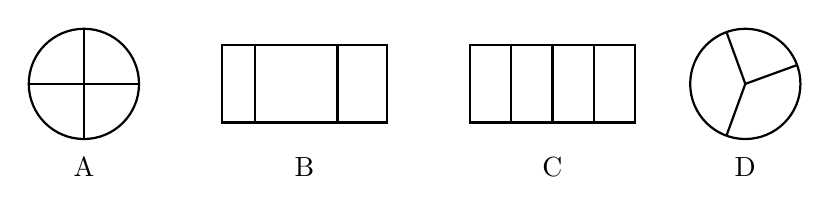
\begin{tikzpicture}[scale=0.7]
\draw[thick] (0,0) circle (1);
\draw[thick] (-1,0)--(1,0);
\draw[thick] (0,-1)--(0,1);
\node at (0,-1.5) {A};
\draw[thick] (2.5,-0.7) rectangle (5.5,0.7);
\draw[thick] (3.1,-0.7)--(3.1,0.7);
\draw[thick] (4.6,-0.7)--(4.6,0.7);
\node at (4,-1.5) {B};
\draw[thick] (7,-0.7) rectangle (10,0.7);
\draw[thick] (7.75,-0.7)--(7.75,0.7);
\draw[thick] (8.5,-0.7)--(8.5,0.7);
\draw[thick] (9.25,-0.7)--(9.25,0.7);
\node at (8.5,-1.5) {C};
\draw[thick] (12,0) circle (1);
\draw[thick] (12,0)--++(20:1);
\draw[thick] (12,0)--++(110:1);
\draw[thick] (12,0)--++(250:1);
\node at (12,-1.5) {D};
\end{tikzpicture}
\end{center}

\wblines{2}

\item Dibuja un rectángulo y divídelo en $4$ partes iguales.

\wbbox[3cm]

\item Dibuja un círculo y traza una línea para dividirlo en $2$ partes iguales.

\wbbox[3cm]

\item Tres amigos comparten una gelatina rectangular. Dibuja cómo la dividirías para que el reparto sea justo.

\wbbox[3cm]

\item Cuatro niños comparten un pastel redondo. Si cada niño recibe una parte, ¿en cuántas partes iguales lo debes cortar? \wbblank

¿Cuántas partes recibe cada niño? \wbblank

\item Explica con tus palabras por qué no es justo repartir una pizza en $2$ partes si una persona recibe una parte más grande que la otra.

\wblines{3}

\item Cierto o falso: ``Si corto un sándwich en $2$ partes y una es más grande, cada parte es una mitad.'' \wbblank[3cm]

Explica tu respuesta.

\wblines{2}
\end{enumerate}
\end{wbpractice}

\section{Mitades, tercios y cuartos}

Toma una tira de papel y dóblala por la mitad, de manera que los dos extremos coincidan exactamente. Al abrirla ves $2$ partes iguales. Cada parte es \textbf{un medio} de la tira.

Ahora dobla la tira por la mitad y, sin abrirla, dóblala otra vez por la mitad. Al abrirla tendrás $4$ partes iguales. Cada parte es \textbf{un cuarto}.

\begin{wbidea}[El nombre de cada parte]
El número de partes iguales le da el nombre a cada parte.

\begin{center}
\wbfracbar[4.5cm]{1}{2} \quad \textbf{un medio} ($2$ partes iguales)\\[1em]
\wbfracbar[4.5cm]{1}{3} \quad \textbf{un tercio} ($3$ partes iguales)\\[1em]
\wbfracbar[4.5cm]{1}{4} \quad \textbf{un cuarto} ($4$ partes iguales)\\[1em]
\wbfracbar[4.5cm]{1}{8} \quad \textbf{un octavo} ($8$ partes iguales)
\end{center}
\end{wbidea}

\begin{wbexample}[Doblar y doblar otra vez]
Dobla una tira de papel por la mitad y, sin abrirla, otra vez por la mitad. Al abrirla, ¿en cuántas partes iguales queda dividida? ¿Cómo se llama cada parte?

\textbf{Paso 1.} El primer doblez divide la tira en $2$ partes iguales.

\textbf{Paso 2.} El segundo doblez divide cada mitad en $2$ partes iguales.

\textbf{Paso 3.} Entonces $2 \times 2 = 4$. Al abrir la tira, queda dividida en $4$ partes iguales.

\textbf{Paso 4.} Cuando hay $4$ partes iguales, cada parte se llama \textbf{un cuarto}. La parte coloreada muestra un cuarto.

\begin{center}
\wbfracbar[6cm]{1}{4}
\end{center}

\textbf{Respuesta:} la tira queda en $4$ partes iguales y cada parte es un cuarto.
\end{wbexample}

\begin{wbexample}[Colorear tres cuartos]
Colorea $\frac{3}{4}$ de esta tira.

\begin{center}
\wbfracbar[6cm]{0}{4}
\end{center}

\textbf{Paso 1.} La tira ya está dividida en $4$ partes iguales, así que cada parte es un cuarto.

\textbf{Paso 2.} El número de arriba es $3$, entonces debo colorear $3$ partes.

\textbf{Paso 3.} Coloreo $3$ de las $4$ partes y dejo $1$ sin colorear.

\begin{center}
\wbfracbar[6cm]{3}{4}
\end{center}

\textbf{Respuesta:} quedan $3$ partes coloreadas de $4$, es decir, $\frac{3}{4}$ de la tira.
\end{wbexample}

\begin{wbexample}[Un tercio del pastel]
Un pastel redondo se corta en $3$ partes iguales. ¿Cómo se llama cada parte?

\textbf{Paso 1.} El pastel está dividido en $3$ partes iguales.

\textbf{Paso 2.} Cuando hay $3$ partes iguales, cada parte se llama \textbf{un tercio}. La parte coloreada muestra un tercio.

\begin{center}
\wbfraccircle{1}{3}
\end{center}

\textbf{Respuesta:} cada parte es un tercio del pastel.
\end{wbexample}

\begin{wbtip}[Cuenta las partes iguales]
Antes de decir el nombre de una parte, cuenta cuántas partes iguales tiene el entero. Si tiene $4$ partes iguales, son cuartos; si tiene $8$ partes iguales, son octavos.
\end{wbtip}

\begin{wbpractice}
\begin{enumerate}
\item Escribe el nombre de la parte coloreada en cada tira.

\begin{center}
\wbfracbar[4.5cm]{1}{2} \quad \wbblank[2.5cm]\\[1em]
\wbfracbar[4.5cm]{1}{3} \quad \wbblank[2.5cm]\\[1em]
\wbfracbar[4.5cm]{1}{4} \quad \wbblank[2.5cm]\\[1em]
\wbfracbar[4.5cm]{1}{8} \quad \wbblank[2.5cm]
\end{center}

\item Colorea un tercio de la tira.

\wbfracbar[6cm]{0}{3}

\item Colorea un cuarto del círculo.

\wbfraccircle{0}{4}

\item Completa: si divido una hoja en $8$ partes iguales, cada parte es un \wbblank[3cm].

\item Colorea la mitad de la cuadrícula.

\wbfracgrid{0}{2}{4}

\item Mamá cortó un pastel en $4$ partes iguales y me dio $1$ parte. ¿Qué parte del pastel recibí? \wbblank[3cm]

\item Dibuja un círculo, divídelo en $3$ partes iguales y colorea una parte. Escribe el nombre de la parte coloreada.

\wbbox[4cm]
\end{enumerate}
\end{wbpractice}

\section{Numerador y denominador}

Ya sabes dividir un entero en partes iguales y nombrar cada parte. Ahora vamos a representar esas partes con números: vamos a escribir \textbf{fracciones}.

\begin{wbidea}[Numerador y denominador]
Una fracción se escribe con dos números separados por una rayita, como $\frac{3}{4}$.

\begin{itemize}
\item El \textbf{denominador} es el número de \emph{abajo}. Dice en cuántas partes iguales se dividió el entero.
\item El \textbf{numerador} es el número de \emph{arriba}. Dice cuántas de esas partes tomamos o coloreamos.
\end{itemize}

\begin{center}
\begin{tikzpicture}[scale=1]
\fill[wbaccent!40] (0,0) rectangle (3,1);
\draw[thick] (0,0) rectangle (4,1);
\draw[thick] (1,0)--(1,1);
\draw[thick] (2,0)--(2,1);
\draw[thick] (3,0)--(3,1);
\node at (2,1.6) {numerador $\rightarrow$ $3$ partes coloreadas};
\node at (2,-0.6) {denominador $\rightarrow$ $4$ partes iguales};
\end{tikzpicture}
\end{center}
\end{wbidea}

\begin{wbexample}[Escribir la fracción de una tira]
¿Qué fracción de la tira está coloreada?

\begin{center}
\wbfracbar[6cm]{3}{4}
\end{center}

\textbf{Paso 1.} Cuento las partes iguales en que está dividida la tira: son $4$. Ese es el \textbf{denominador}.

\textbf{Paso 2.} Cuento las partes coloreadas: son $3$. Ese es el \textbf{numerador}.

\textbf{Paso 3.} Escribo el numerador arriba y el denominador abajo: $\frac{3}{4}$.

\textbf{Paso 4.} Lo leo: ``tres cuartos''.

\textbf{Respuesta:} $\frac{3}{4}$ de la tira está coloreada.
\end{wbexample}

\begin{wbexample}[Escribir la fracción de un círculo]
¿Qué fracción del círculo está coloreada?

\begin{center}
\wbfraccircle{5}{8}
\end{center}

\textbf{Paso 1.} Cuento todas las partes iguales del círculo: son $8$. El denominador es $8$.

\textbf{Paso 2.} Cuento las partes coloreadas: son $5$. El numerador es $5$.

\textbf{Paso 3.} Escribo la fracción: $\frac{5}{8}$.

\textbf{Paso 4.} Lo leo: ``cinco octavos''.

\textbf{Respuesta:} $\frac{5}{8}$ del círculo está coloreado.
\end{wbexample}

\begin{wbexample}[Colorear una fracción de una cuadrícula]
Colorea $\frac{3}{8}$ de la cuadrícula.

\begin{center}
\wbfracgrid{0}{2}{4}
\end{center}

\textbf{Paso 1.} El denominador es $8$, así que la cuadrícula debe tener $8$ partes iguales. La cuadrícula tiene $2$ filas de $4$ cuadritos, es decir, $2 \times 4 = 8$ partes iguales.

\textbf{Paso 2.} El numerador es $3$, así que coloreo $3$ partes.

\textbf{Paso 3.} Coloreo $3$ cuadritos y dejo $5$ sin colorear.

\begin{center}
\wbfracgrid{3}{2}{4}
\end{center}

\textbf{Respuesta:} $3$ cuadritos coloreados de $8$, es decir, $\frac{3}{8}$.
\end{wbexample}

\begin{wbtip}[Cómo se lee una fracción]
No leas $\frac{3}{4}$ como ``tres cuatro''. Se lee \textbf{tres cuartos}: primero el numerador y luego el nombre de las partes.

Si el entero se divide en $5$ partes iguales, cada parte es un \textbf{quinto}. Si se divide en $6$ partes iguales, cada parte es un \textbf{sexto}.
\end{wbtip}

\begin{wbpractice}
\begin{enumerate}
\item ¿Qué fracción de la tira está coloreada? Escribe la fracción y cómo se lee.

\begin{center}
\wbfracbar[6cm]{2}{5}
\end{center}

\wbfracbox \quad Se lee: \wbblank[4cm]

\item ¿Qué fracción del círculo está coloreada?

\begin{center}
\wbfraccircle{1}{3}
\end{center}

\wbfracbox

\item ¿Qué fracción de la cuadrícula está coloreada?

\begin{center}
\wbfracgrid{5}{2}{4}
\end{center}

\wbfracbox

\item Colorea $\frac{2}{3}$ de la tira.

\wbfracbar[6cm]{0}{3}

\item Completa la tabla.

\begin{center}
\begin{tabular}{|c|c|c|}
\hline
Fracción & Numerador & Denominador \\
\hline
$\frac{3}{4}$ & \wbblank[1.5cm] & \wbblank[1.5cm] \\
\hline
$\frac{5}{8}$ & \wbblank[1.5cm] & \wbblank[1.5cm] \\
\hline
\end{tabular}
\end{center}

\item Una sandía se dividió en $6$ rebanadas iguales. Lupita comió $2$ rebanadas. ¿Qué fracción de la sandía comió?

\wbfracbox

\item Explica con tus palabras qué indica el numerador de una fracción.

\wblines{3}

\item Escribe cómo se lee la fracción $\frac{5}{8}$: \wbblank[4cm]
\end{enumerate}
\end{wbpractice}

\begin{wbreview}
\begin{enumerate}
\item Observa las figuras. Escribe las letras de las que están divididas en partes iguales.

\begin{center}
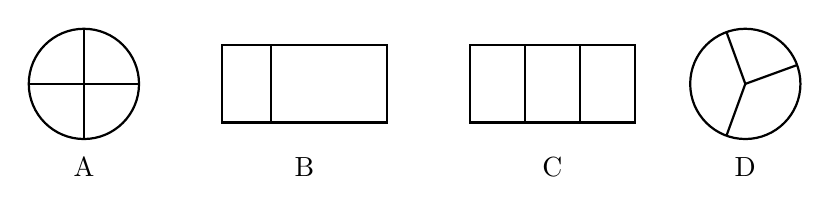
\begin{tikzpicture}[scale=0.7]
\draw[thick] (0,0) circle (1);
\draw[thick] (-1,0)--(1,0);
\draw[thick] (0,-1)--(0,1);
\node at (0,-1.5) {A};
\draw[thick] (2.5,-0.7) rectangle (5.5,0.7);
\draw[thick] (3.4,-0.7)--(3.4,0.7);
\node at (4,-1.5) {B};
\draw[thick] (7,-0.7) rectangle (10,0.7);
\draw[thick] (8,-0.7)--(8,0.7);
\draw[thick] (9,-0.7)--(9,0.7);
\node at (8.5,-1.5) {C};
\draw[thick] (12,0) circle (1);
\draw[thick] (12,0)--++(20:1);
\draw[thick] (12,0)--++(110:1);
\draw[thick] (12,0)--++(250:1);
\node at (12,-1.5) {D};
\end{tikzpicture}
\end{center}

\wblines{2}

\item Dibuja un rectángulo y divídelo en $4$ partes iguales.

\wbbox[3cm]

\item ¿Qué fracción de la tira está coloreada?

\begin{center}
\wbfracbar[6cm]{3}{4}
\end{center}

\wbfracbox

\item Colorea $\frac{1}{2}$ del círculo.

\wbfraccircle{0}{2}

\item Completa: en la fracción $\frac{5}{8}$, el numerador es \wbblank y el denominador es \wbblank.

\item Cuatro amigos se reparten por igual una barra de chocolate dividida en $4$ partes iguales. ¿Qué parte del chocolate recibe cada uno? \wbblank[3cm]

\item Escribe cómo se lee la fracción $\frac{2}{3}$: \wbblank[4cm]

\item Explica con tus palabras qué es una fracción.

\wblines{3}
\end{enumerate}
\end{wbreview}
%%% END UNIT
%%% BEGIN ANSWERS
\wbanswers{\wbLPractice\ 1.1}
\begin{enumerate}
\item A y C. Cada una tiene $4$ partes iguales; B y D tienen partes de distinto tamaño.
\item Un rectángulo dividido en $4$ partes iguales; por ejemplo, con $3$ líneas verticales igualmente espaciadas.
\item Un círculo con una línea recta que pasa por su centro y une dos puntos de su borde.
\item Un rectángulo dividido en $3$ partes iguales.
\item En $4$ partes iguales; cada niño recibe $1$ parte.
\item Porque una persona recibe más que la otra. Para que sea justo, las dos partes deben tener el mismo tamaño.
\item Falso. Las partes no son iguales, así que ninguna es una mitad del sándwich.
\end{enumerate}

\wbanswers{\wbLPractice\ 1.2}
\begin{enumerate}
\item Un medio; un tercio; un cuarto; un octavo.
\item Colorear $1$ de las $3$ partes.
\item Colorear $1$ de las $4$ partes.
\item Octavo.
\item Colorear $4$ de los $8$ cuadritos.
\item Un cuarto del pastel.
\item Un círculo dividido en $3$ partes iguales con $1$ coloreada; escribir ``un tercio''.
\end{enumerate}

\wbanswers{\wbLPractice\ 1.3}
\begin{enumerate}
\item $\frac{2}{5}$; ``dos quintos''.
\item $\frac{1}{3}$.
\item $\frac{5}{8}$.
\item Colorear $2$ de las $3$ partes.
\item $\frac{3}{4}$: numerador $3$, denominador $4$. $\frac{5}{8}$: numerador $5$, denominador $8$.
\item $\frac{2}{6}$ de la sandía.
\item Indica cuántas de las partes iguales del entero tomamos o coloreamos.
\item ``Cinco octavos''.
\end{enumerate}

\wbanswers{\wbLReview}
\begin{enumerate}
\item A y C. A tiene $4$ partes iguales y C tiene $3$; B y D tienen partes desiguales.
\item Un rectángulo dividido en $4$ partes del mismo tamaño.
\item $\frac{3}{4}$.
\item Colorear $1$ de las $2$ partes del círculo.
\item Numerador $5$; denominador $8$.
\item $\frac{1}{4}$ del chocolate.
\item ``Dos tercios''.
\item Una fracción es un número que puede representar partes iguales de un entero. El denominador indica en cuántas partes iguales se dividió y el numerador, cuántas se toman.
\end{enumerate}
%%% END ANSWERS